\documentclass[letterpaper]{article}
\usepackage[utf8]{inputenc}
\usepackage[spanish]{babel}
\usepackage[pdftex]{graphicx}
\usepackage{amssymb}
\usepackage{amsmath}
\usepackage{url}
\usepackage{slashbox}


\usepackage[pdftitle={complementos de informatica},
			pdfauthor={Insaurralde},
			pdfkeywords={ paraguay}
		   ]{hyperref}
		   
\hypersetup{
    colorlinks,
    citecolor=black,
    filecolor=black,
    linkcolor=black,
    urlcolor=black
}

\newcommand{\HRule}{\rule{\linewidth}{0.5mm}}

\setcounter{tocdepth}{3}
\makeatletter

\title{Complementos de Informatica}
\author{Insaurralde}

\makeatletter
\g@addto@macro{\UrlBreaks}{\UrlOrds}
\makeatother

\begin{document}

	\begin{titlepage}
		\begin{center}
			
\includegraphics[width=0.5\textwidth]{img/logo_uca.jpg}\\[1cm]    
			\textsc{\LARGE Redes de Computadora I}\\[1.5cm]


			% Titulo
			\HRule \\[0.4cm]
			{ \huge \bfseries 
Laboratorio II - Investigación con sniffer Wireshark }\\[0.4cm]
			\HRule \\[0.4cm]

			% Autor y Supervisor
			\begin{minipage}{0.4\textwidth}
				\begin{flushleft} \large
					\emph{Autor:} \\ \textsc{Ramon Insaurralde}
				\end{flushleft}
			\end{minipage}
		
			\vfill
		\begin{abstract}
				
Desarrollaremos un análisis del comportamiento de la red en diferentes situaciones, elaboraremos un resúmen de los protocolos, servicios y puertos al utilizar la red gracias a la herramienta tipo sniffer llamada wireshark, para este trabajo usaremos la red wiffi para hacer todas las pruebas. 		
			\end{abstract}

		\end{center}
	\end{titlepage}

	\tableofcontents
	\newpage
	\section{Introducción}
Wireshark, antes conocido como Ethereal, es un analizador de protocolos utilizado para realizar análisis y solucionar problemas en redes de comunicaciones, para desarrollo de software y protocolos, y como una herramienta didáctica. Cuenta con todas las características estándar de un analizador de protocolos de forma únicamente hueca.
La funcionalidad que provee es similar a la de tcpdump, pero añade una interfaz gráfica y muchas opciones de organización y filtrado de información. Así, permite ver todo el tráfico que pasa a través de una red (usualmente una red Ethernet, aunque es compatible con algunas otras) estableciendo la configuración en modo promiscuo. También incluye una versión basada en texto llamada tshark.
Permite examinar datos de una red viva o de un archivo de captura salvado en disco. Se puede analizar la información capturada, a través de los detalles y sumarios por cada paquete. Wireshark incluye un completo lenguaje para filtrar lo que queremos ver y la habilidad de mostrar el flujo reconstruido de una sesión de TCP.

		
	
\section{Marco teórico}
En este trabajo realizaremos la siguiente actividad, capturar paquetes de la red cuando se da:\\
i. Login http. \\
ii. Login https. \\
iii. Consulta de un dominio a un DNS.\\ 
iv. Envio de un email. \\
v. Descarga de archivos P2P.\\ 
vi. Intercambio de paquetes para conectarse a una red WiFi segura. \\
vii. Intercambio de paquetes para conexión DHCP. \\

Obs: Ademas de capturar los paquetes se debe analizar el contenido del paquete dando explicaciones sobre cada uno de ellos.

\section{Análisis de los resultados}
En esta sección analizaremos insitu los comportamientos del capturador de paquetes para los casos solicitados por la investigación, cada Item contará con imágenes que apoyaran el proceso explicativo.

\newpage
\subsection{Login HTTP}
	\begin{figure}[h]
			\centering
			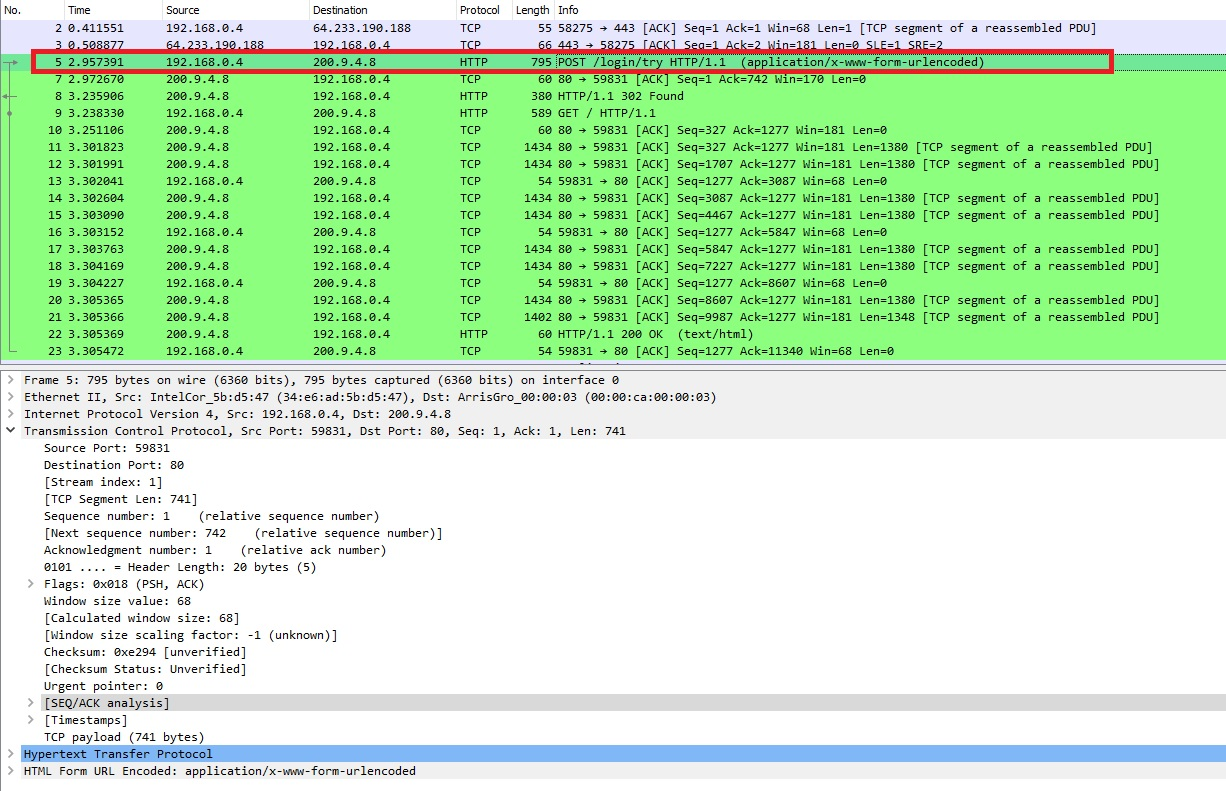
\includegraphics[width=0.9\textwidth]{img/http-login-1.jpg}
			\caption{Login HTTP-WIRESHARK}
			\label{figura 1}
		\end{figure}



\subsubsection{Explicación}
\paragraph{En la figura 1 podemos observar en verde los paquetes que se intercambian entre el servidor de sapienza ( ip 200.9.4.8) y la máquina que utilizamos como prueba (ip 192.168.0.4 local). Al realizar el procedimiento de login, se realizan una serie de intercambios de paquetes, la mayoria de ellos de ack e información emitida y recibida por partes dentro de los envios. Al inicio se envian usuario y password no encriptado (ver figura 2).}

\begin{figure}[h]
	\centering
	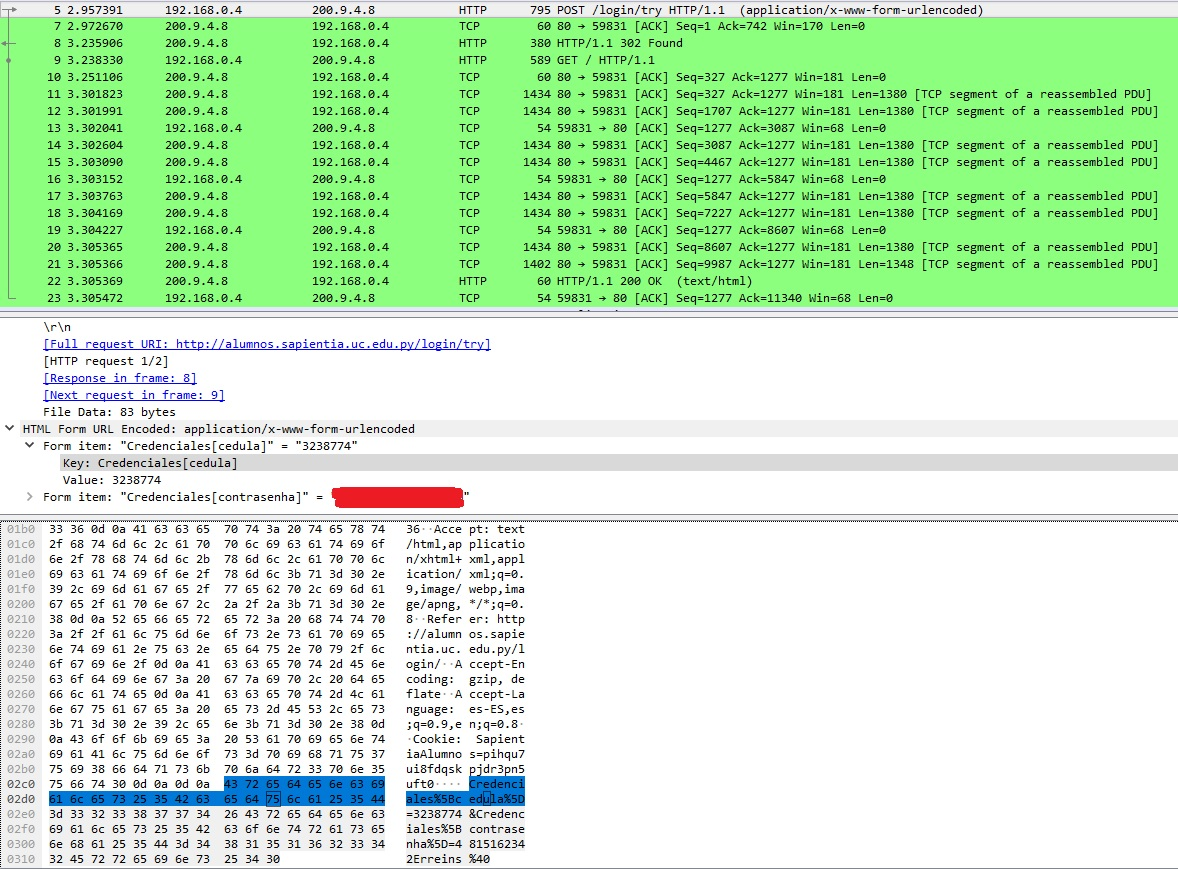
\includegraphics[width=0.9\textwidth]{img/http-login-5.jpg}
	\caption{Login HTTP-WIRESHARK-Login y Password}
	\label{figura 2}
\end{figure}

\newpage

\begin{figure}[h]
	\centering
	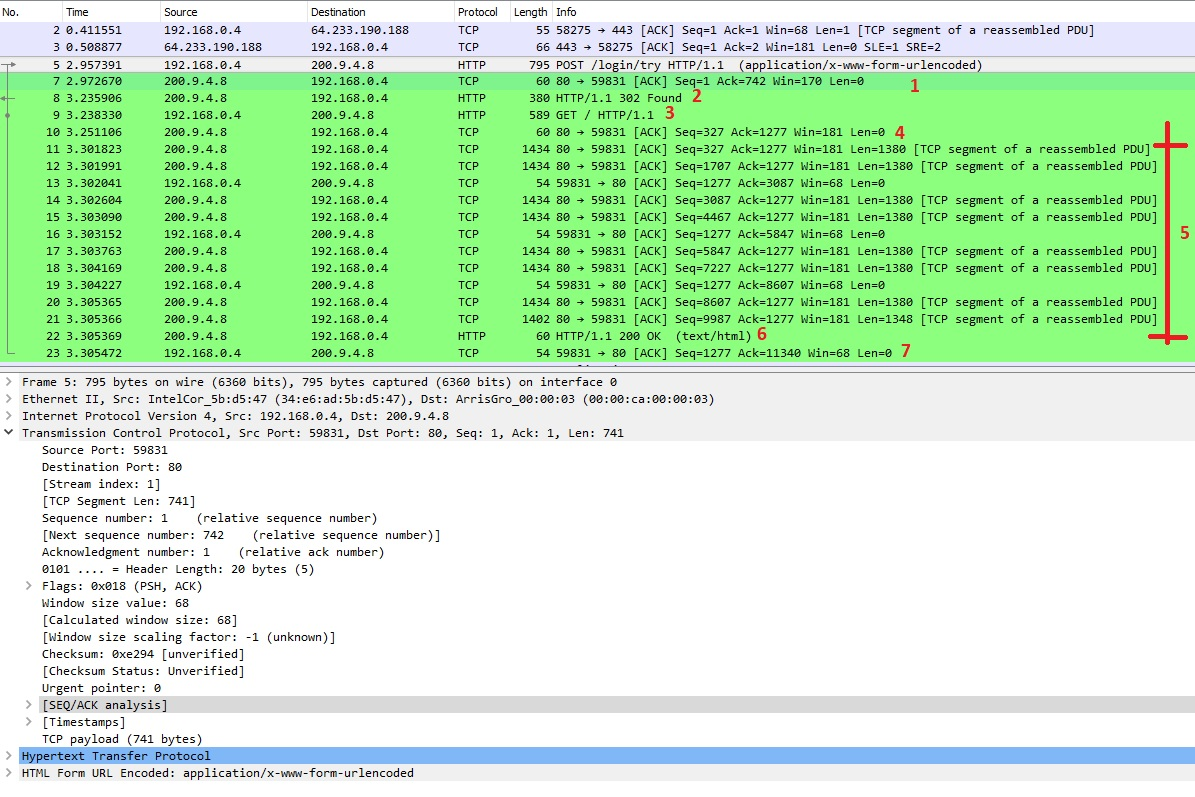
\includegraphics[width=0.9\textwidth]{img/http-login-2.jpg}
	\caption{Login HTTP-WIRESHARK}
	\label{figura 3}
\end{figure}

\paragraph{Descripción Paso a Paso (FIGURA 3):}

	\begin{itemize}
				
		\item{1: Solicitud de conexión del puerto 59831 al puerto 80 de Sapienza, Método: POST comando: login/try protocolo: HTTP/1.1  }

		\item{2: Confirmación HTTP/1.1 de protocolo, servidor CENTOS, apache 2.2.15, php-version: 5.5.36, }
		\item{3: Protocolo: HTTP Metodo: GET, Url: / en este caso el servidor da la posibilidad de recibir el url al cual conectarse por parte del navegador, }
		\item{4: El navegador envia un ACK aceptando el GET, del puerto 80 al 59831}
		\item{5: Serie de intercambio de paquetes de información, la fuente envia paquetes con dimensiones iguales y el servidor responde con ACK cada dos envios, al principio supucimos que eran errores de envio vista la periodicidad y dimensión, luego llegamos a la conclusión de que Wireshark ha concatenado una serie de segmentos mostrando en el toda la información completa.No se trata de ningún error}
		\item{6: El servidor aceptó la información enviada, el mismo responde con un codigo HTTP/1.1 numero 200, el cual indica que la información enviada corresponde a un usuario, el mismo envia en su sección text data una página web completa, de tipo text/html con la información del alumno en este caso.}
		\item{7: ACK de recepción por parte del la computadora de prueba, ambos servidores dejan de enviarse por el momento paquetes ya que el protocolo de login finalizó con éxito. }
	\end{itemize}
\subsection{Login HTTPS}

\begin{figure}
	\centering
	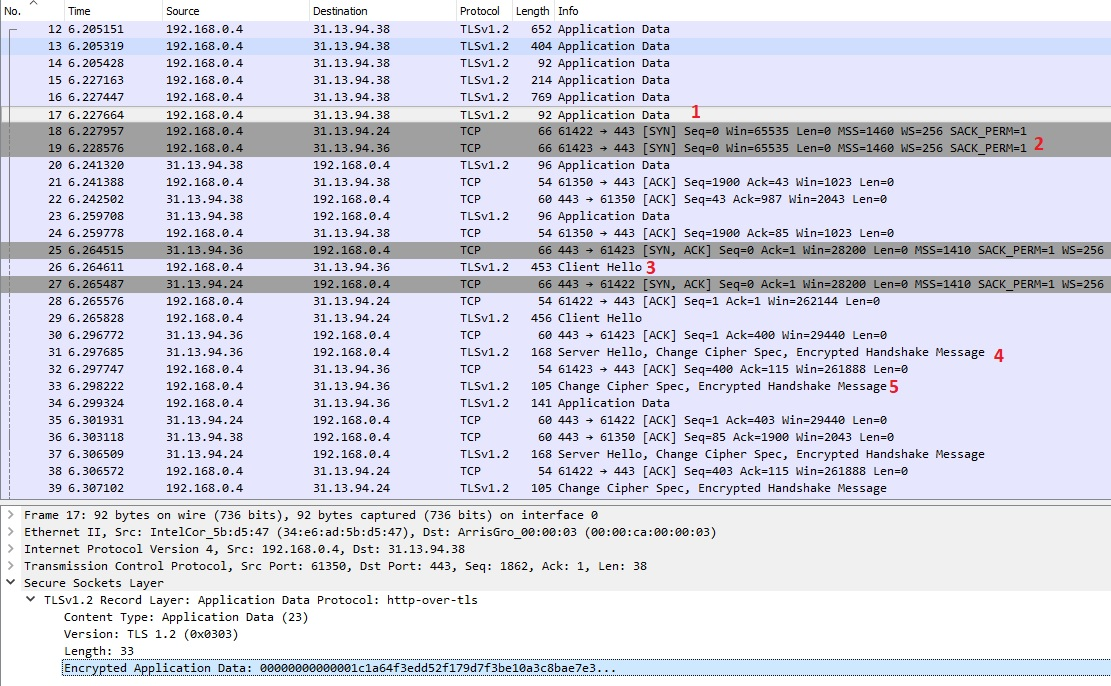
\includegraphics[width=0.9\textwidth]{img/https-login-1.jpg}
	\caption{Login HTTPS-WIRESHARK}
	\label{figura 4}
\end{figure}	

\subsubsection{Explicación}
\paragraph{En la figura 4 observamos los paquetes intercambiados por la fuente, mi computadora, con ip (192.168.0.4 local) y el servidor web (31.13.94.38), al realizarse un login bajo el protocolo HTTPS (TLSV1.2), podemos observar a priori que el primer procedimiento que intenta realizar la fuente desde el puerto 61350 al puerto 443 del servidor es tratar de enviar la información encriptada al mismo. Podemos observar que la información que anteriormente vimos estaba pasada directamente con el LOGIN HTTP, ahora esta encriptada y se pasa a traves del protocolo TLS v 1.2 (ver figura 4)}

\paragraph{Descripción Paso a Paso (FIGURA 4):}
\begin{itemize}
				
\item{1: Intento de envío de información encriptada al servidor, app-data-protocol: http-over-tls; Src Port: 61350; Dst Port: 443; }

\item{2:En este caso el servidor host, envia un paquete SYN al servidor de Destino, el mismo responde con un paguete SYN nuevamente, en este paso inicia lo que se denomina como HeandSHake entre la fuente y el Destino. Lo importante es señalar el proceso de conocido para que se realize una conexión socket tcp \\
El host A envía un paquete TCP SYNchronize al Host B \\
El anfitrión B recibe el SYN de A \
El anfitrión B envía un reconocimiento SYNchronize \\
El anfitrión A recibe el SYN-ACK de B \\
El anfitrión A envía ACKnowledge \\
El anfitrión B recibe ACK. \\
La conexión de socket TCP está ESTABLISHED. \\
}
\item{3,4 y 5: En estos pasos se explica como funciona el  Protocolo de TLS Handshake el cual implica los siguientes pasos:\\
1- El cliente envía un mensaje (Client hello) al servidor, junto con el valor aleatorio del cliente y las suites de cifrado(clipher suites) admitidas.\\
2- El servidor responde enviando un mensaje (Server Hello) al cliente, junto con el valor aleatorio del servidor.\\
3- El servidor envía su certificado al cliente para la autenticación y puede solicitar un certificado del cliente. El servidor envía el mensaje (Servidor hello done).\\
4- Si el servidor ha solicitado un certificado del cliente, el cliente lo envía.\\
5- El cliente crea un Pre-Master Secret aleatorio y lo encripta con la clave pública del certificado del servidor, enviando el Pre-Master Secret encriptado al servidor.\\
6- El servidor recibe el secreto Pre-Master. El servidor y el cliente generan el secreto principal y las claves de sesión basadas en el secreto premaster.\\
7- El cliente envía la notificación (Cambiar especificación de cifrado) al servidor para indicar que el cliente comenzará a utilizar las nuevas claves de sesión para el hash y el cifrado de mensajes. El cliente también envía un mensaje de (Cliente terminado).\\
8- El servidor recibe (Cambiar especificación de cifrado) y cambia su estado de seguridad de la capa de registro a cifrado simétrico utilizando las claves de sesión. El servidor envía el mensaje (Servidor terminado) al cliente.\\
9- El cliente y el servidor ahora pueden intercambiar datos de aplicaciones a través del canal seguro que han establecido. Todos los mensajes enviados de cliente a servidor y de servidor a cliente se cifran mediante la clave de sesión.\\ }

\end{itemize}

\subsection{Consulta de un dominio DNS}



\paragraph{Para realizar este procedimiento, debemos hacer ping a un dominio cualquiera, como por ejemplo google.com y ver los paquetes asociados al momento de realizar la consulta al dominio.}

\subsubsection{Explicación}
\paragraph{La figura 5 se  muestra los paquetes filtrados para la dirección ip de origen, la consulta en cuestión corresponde a un PING al dominio www.google.com }
\begin{itemize}
				
\item{1: Consulta desde la ip de origen, a la ip del DNS con la consulta especifica, la consulta origen sale del puerto 60181 al puerto 53 del servidor DNS; la consulta(query) simplemente contiene el nombre de dominio y el tipo de consulta en este caso es A (address), y la clase que es IN(internet), en la segunda linea, el servidor DNS responde(answere) al host origen con lo siguiente: toda la info requerida al inicio mas la dirección IP de la dirección requerida. en este caso es: 216.58.202.4 (ver figura 6)}


\item{2: A traves del protocolo ICMP(internet control message protocol) el host envia y recibe paquetes del servidor de google en este caso, estos mensajes simplemente contienen un request y un reply en los cuales los numeros de secuencia tanto para request y reply son los mismos, es un ida-verificación-respuesta continua de 3 paquetes. }

				\end{itemize}
\newpage
\begin{figure}[h]
	\centering
	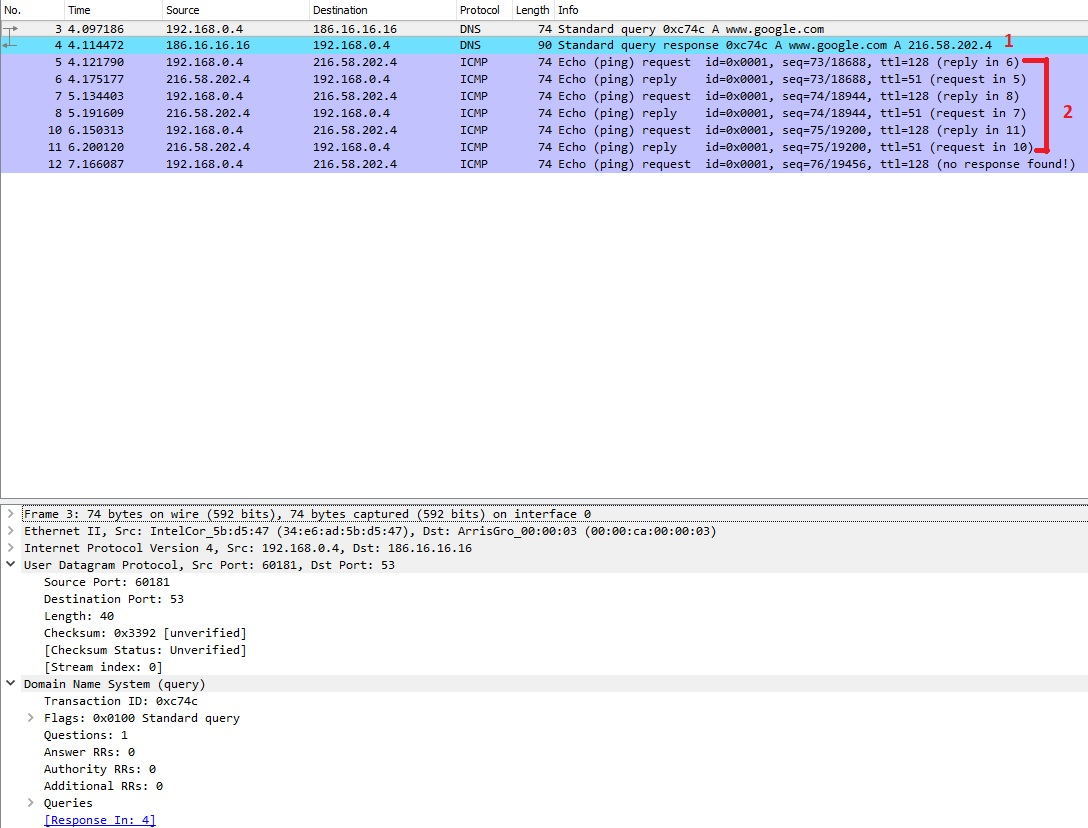
\includegraphics[width=0.9\textwidth]{img/dns-1.jpg}
	\caption{Consulta DNS-WIRESHARK}
	\label{figura 5}
\end{figure}

\paragraph{En la figura 6 Podemos observar como se comporta el servidor DNS al dar una respuesta de localización de la IP del host solicitado }

\begin{figure}[h]
	\centering
	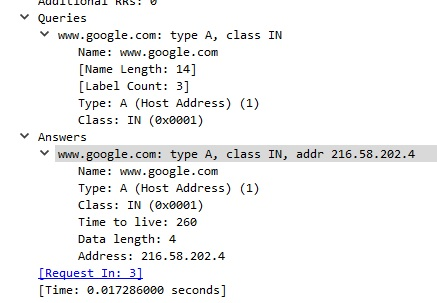
\includegraphics[width=0.5\textwidth]{img/dns-2.jpg}
	\caption{Consulta DNS-Query-Answere-WIRESHARK}
	\label{figura 6}
\end{figure}

\newpage

\subsection{Envio de Email}

\paragraph{En este procedimiento capturaremos los paquetes al realizar un envio de email desde un cliente web de la maquina host, visto que no tenemos un servidor de correo habilitado incitu, veremos como se realiza el proceso de envio desde el cliente de correos de windows.}

\subsubsection{Explicación}
\paragraph{Analizaremos el procedimiento de captura, primero verificando que todos los procedimientos de envío desde servidores web como google, microsoft, etc se realizan a través de protocolos Seguros, osea, utilian TLS v.1.2 como protocolo de conexión socket con el servidor y asi envian la información a través del canal seguro pre-establecido (Ver figura 7 - label intro). Luego Procedimos al análisis de los paquetes tanto enviados y recibidos, y nos dimos cuenta de que:}
\begin{itemize}
				
\item{1: La conexión socket con el servidor es segura, para envios }
\item{2: Errores de retransmisión entre el servidor host y el servidor de microsoft mail}
\item{3: Errores en donde el protocolo avisa algunos errores de transmisión en cuanto a ACK duplicados al momento del envio del mail}

\paragraph{Desde el momento de no tener un servidor de correos propio, fue complicado aplicar los conocimientos al realizar este item en especifico.}			


				\end{itemize}



\begin{figure}[h]
	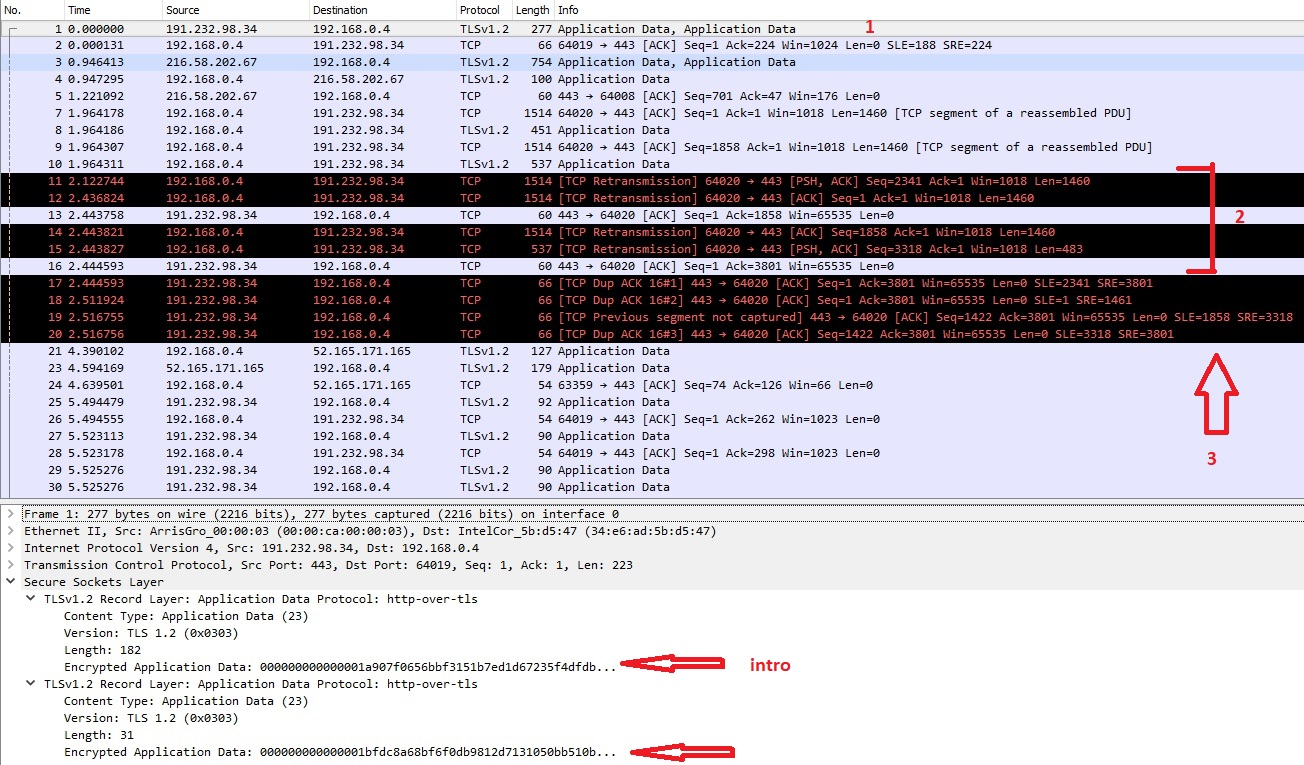
\includegraphics[width=0.9\textwidth]{img/mail-1.jpg}
	\caption{Envio de email}
	\label{figura 7}
\end{figure}
\newpage

\subsection{Descarga de archivos P2P}
\paragraph{En esta sección analizaremos los paquetes que se reciben y envian en el proceso de descarga de archivos a través de la herramienta bittorrent que usa el protocolo p2p. (ver figura 8)}


\begin{figure}[h]
	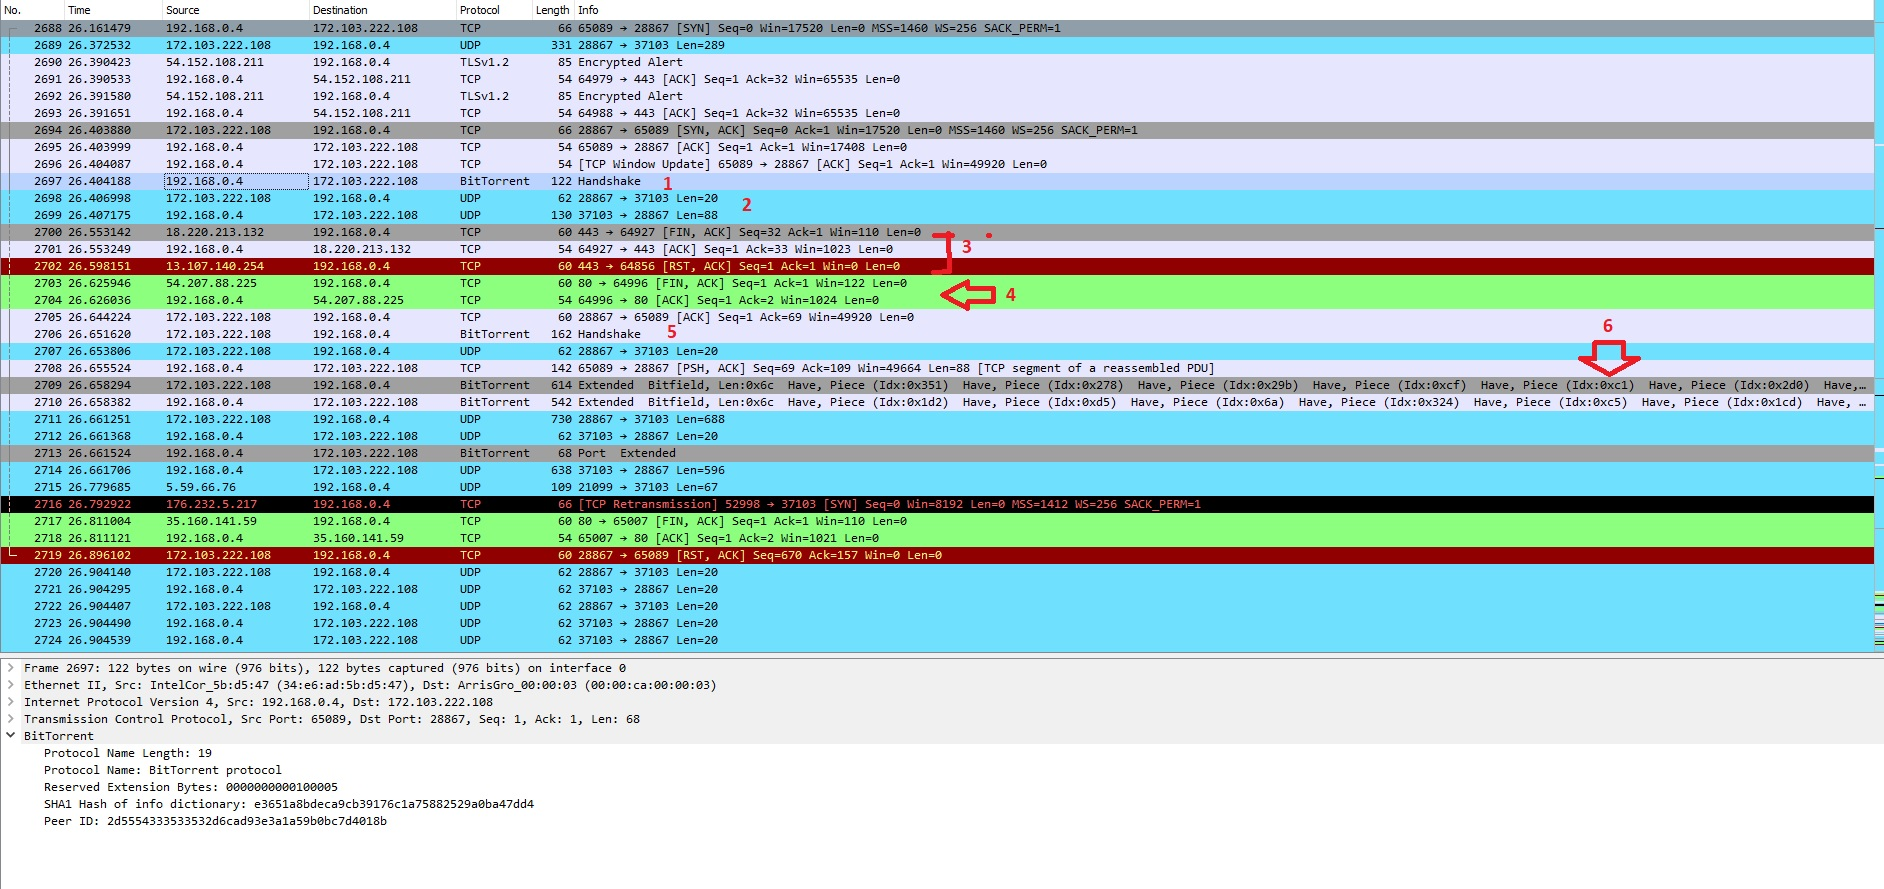
\includegraphics[width=0.9\textwidth]{img/p2p-1.jpg}
	\caption{P2P-DOwnload File}
	\label{figura 8}
\end{figure}

\begin{itemize}
				
\item{1: Handshake entre el servidor de torrent y el host, a traves del protocolo Bitorrent, en esta sección solo se realiza una solicitud unidireccional, se pueden observar que los puertos que utilizan son muy diferentes a los que normalmente conocemos para intercambio de paquetes. }
\item{2: Envio de paquetes a través de protocolo UDP del servidor luego de recibir el handshake, el host a traves del programa responde con un ok por el mismo protocolo }
\item{3 y 4: a traves del protocolo TCP simplemente envio y recepción y finalización de ACK's}
\item{5: Respuesta de Handshake con el mismo protocolo BitTottent}

			\end{itemize}


\subsection{Intercambio de paquetes para conectarse a una red wifi segura}

\paragraph{Hemos realizado las capturas al conectarse a una red wifi previamente conocida. }

\begin{figure}[h]
	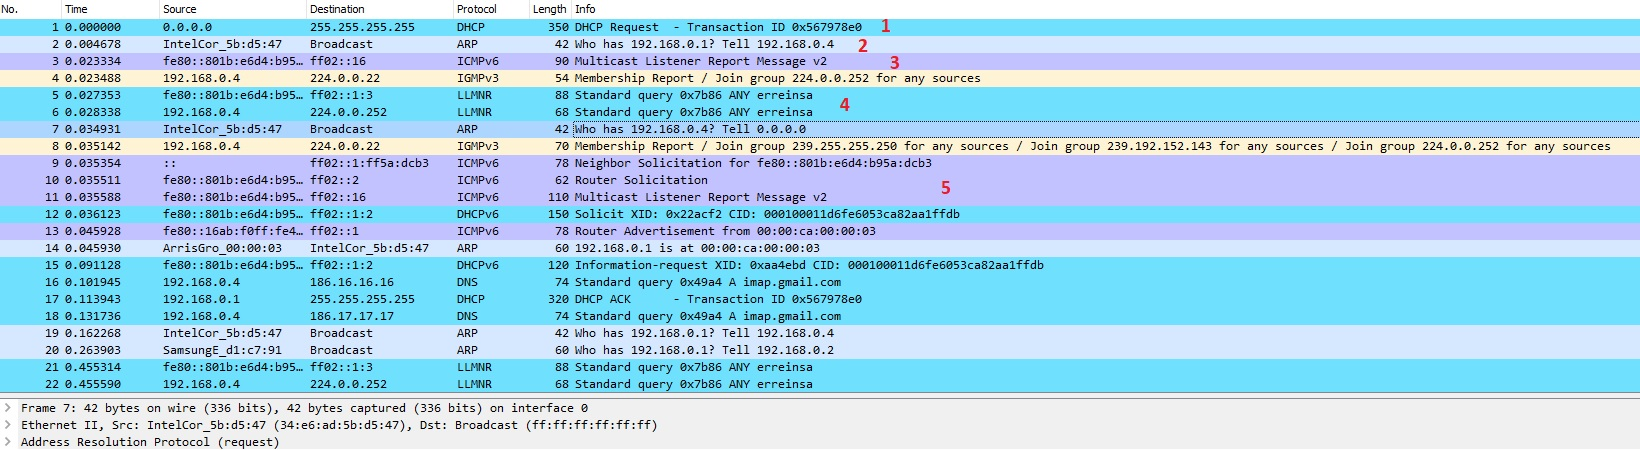
\includegraphics[width=0.9\textwidth]{img/login-wifi-1.jpg}
	\caption{Login Wifi }
	\label{figura 9}
\end{figure}

\begin{itemize}


\subsubsection{Explicación}
				
		\item{1:DHCP request, El cliente pide una dirección IP al host, el mismo utiliza el protocolo dhcp, en el ejemplo de la figura 9, el cliente envia como cabecera el mac address correspondiente a si mismo, recibe una dirección IP.}

\item{2:Identificador del router destino.}
\item{3: El protocolo ICMPv6  es una nueva versión de ICMP y es una parte importante de la arquitectura IPv6 que debe estar completamente soportada por todas las implementaciones y nodos IPv6}
\item{4:La resolución de nombre de multidifusión local de enlace (LLMNR) es un protocolo basado en el formato de paquete de sistema de nombres de dominio (DNS) que permite que los hosts IPv4 e IPv6 realicen la resolución de nombre para hosts en el mismo enlace local.}
\item{5: El protocolo de red IGMP se utiliza para intercambiar información acerca del estado de pertenencia entre enrutadores IP que admiten la multidifusión y miembros de grupos de multidifusión. Los hosts miembros individuales informan acerca de la pertenencia de hosts al grupo de multidifusión y los enrutadores de multidifusión sondean periódicamente el estado de la pertenencia.}


				\end{itemize}
\subsection{Intercambio de paquetes para conexion DHCP}
\paragraph{Hemos mostrado en el item anterior, al conectarse a la red wifi como el protocolo DHCP funciona y que paquetes se intercambian con el host que requiere la ip.}






\end{document}








